\section{Comparison with NuWro and GiBUU}
\label{app:nugen}

In addition to \genie, other dedicated event generators are widely used by the neutrino community.
%
To highlight the flexibility of the pipeline assembled in this work, here we compare \genie with two other generators tailored to neutrino-nucleus scattering, namely {\sc\small NuWro}~\cite{Golan:2012rfa,Juszczak:2009qa} and {\sc\small GiBUU}~\cite{Buss:2011mx}, whose events are processed by the same analysis chain as those of the other generators of Table~\ref{tab:generators}.
%
With this motivation, Fig.~\ref{fig:nugen} displays differential distributions in $x_{\rm Bj}$, $y$, charged-hadron multiplicity $N_{\rm ch}$, and proton multiplicity $N_p$ evaluated in muon-neutrino CC scattering at $E_\nu=200$~GeV in the fiducial region of this benchmark, both on a free proton  target and on a tungsten target.
  %
Predictions from three different neutrino MC event generators are compared: \genie (both default {\tt G18\_02a} tune and {\sc\small HEDIS} tune), {\sc\small NuWro} and {\sc\small GiBUU}.
%
On tungsten, each generator applies its own nuclear model, and the DIS kinematic variables are defined with respect to the struck nucleon.
%
Note that {\sc\small GiBUU} is shown for the free proton only, since its tungsten transport does not complete at $E_\nu=200$ GeV.

%%%%%%%%%%%%%%%%%%%%%%%%%%%%%%%%%
\begin{figure}[!tbp]
  \centering
  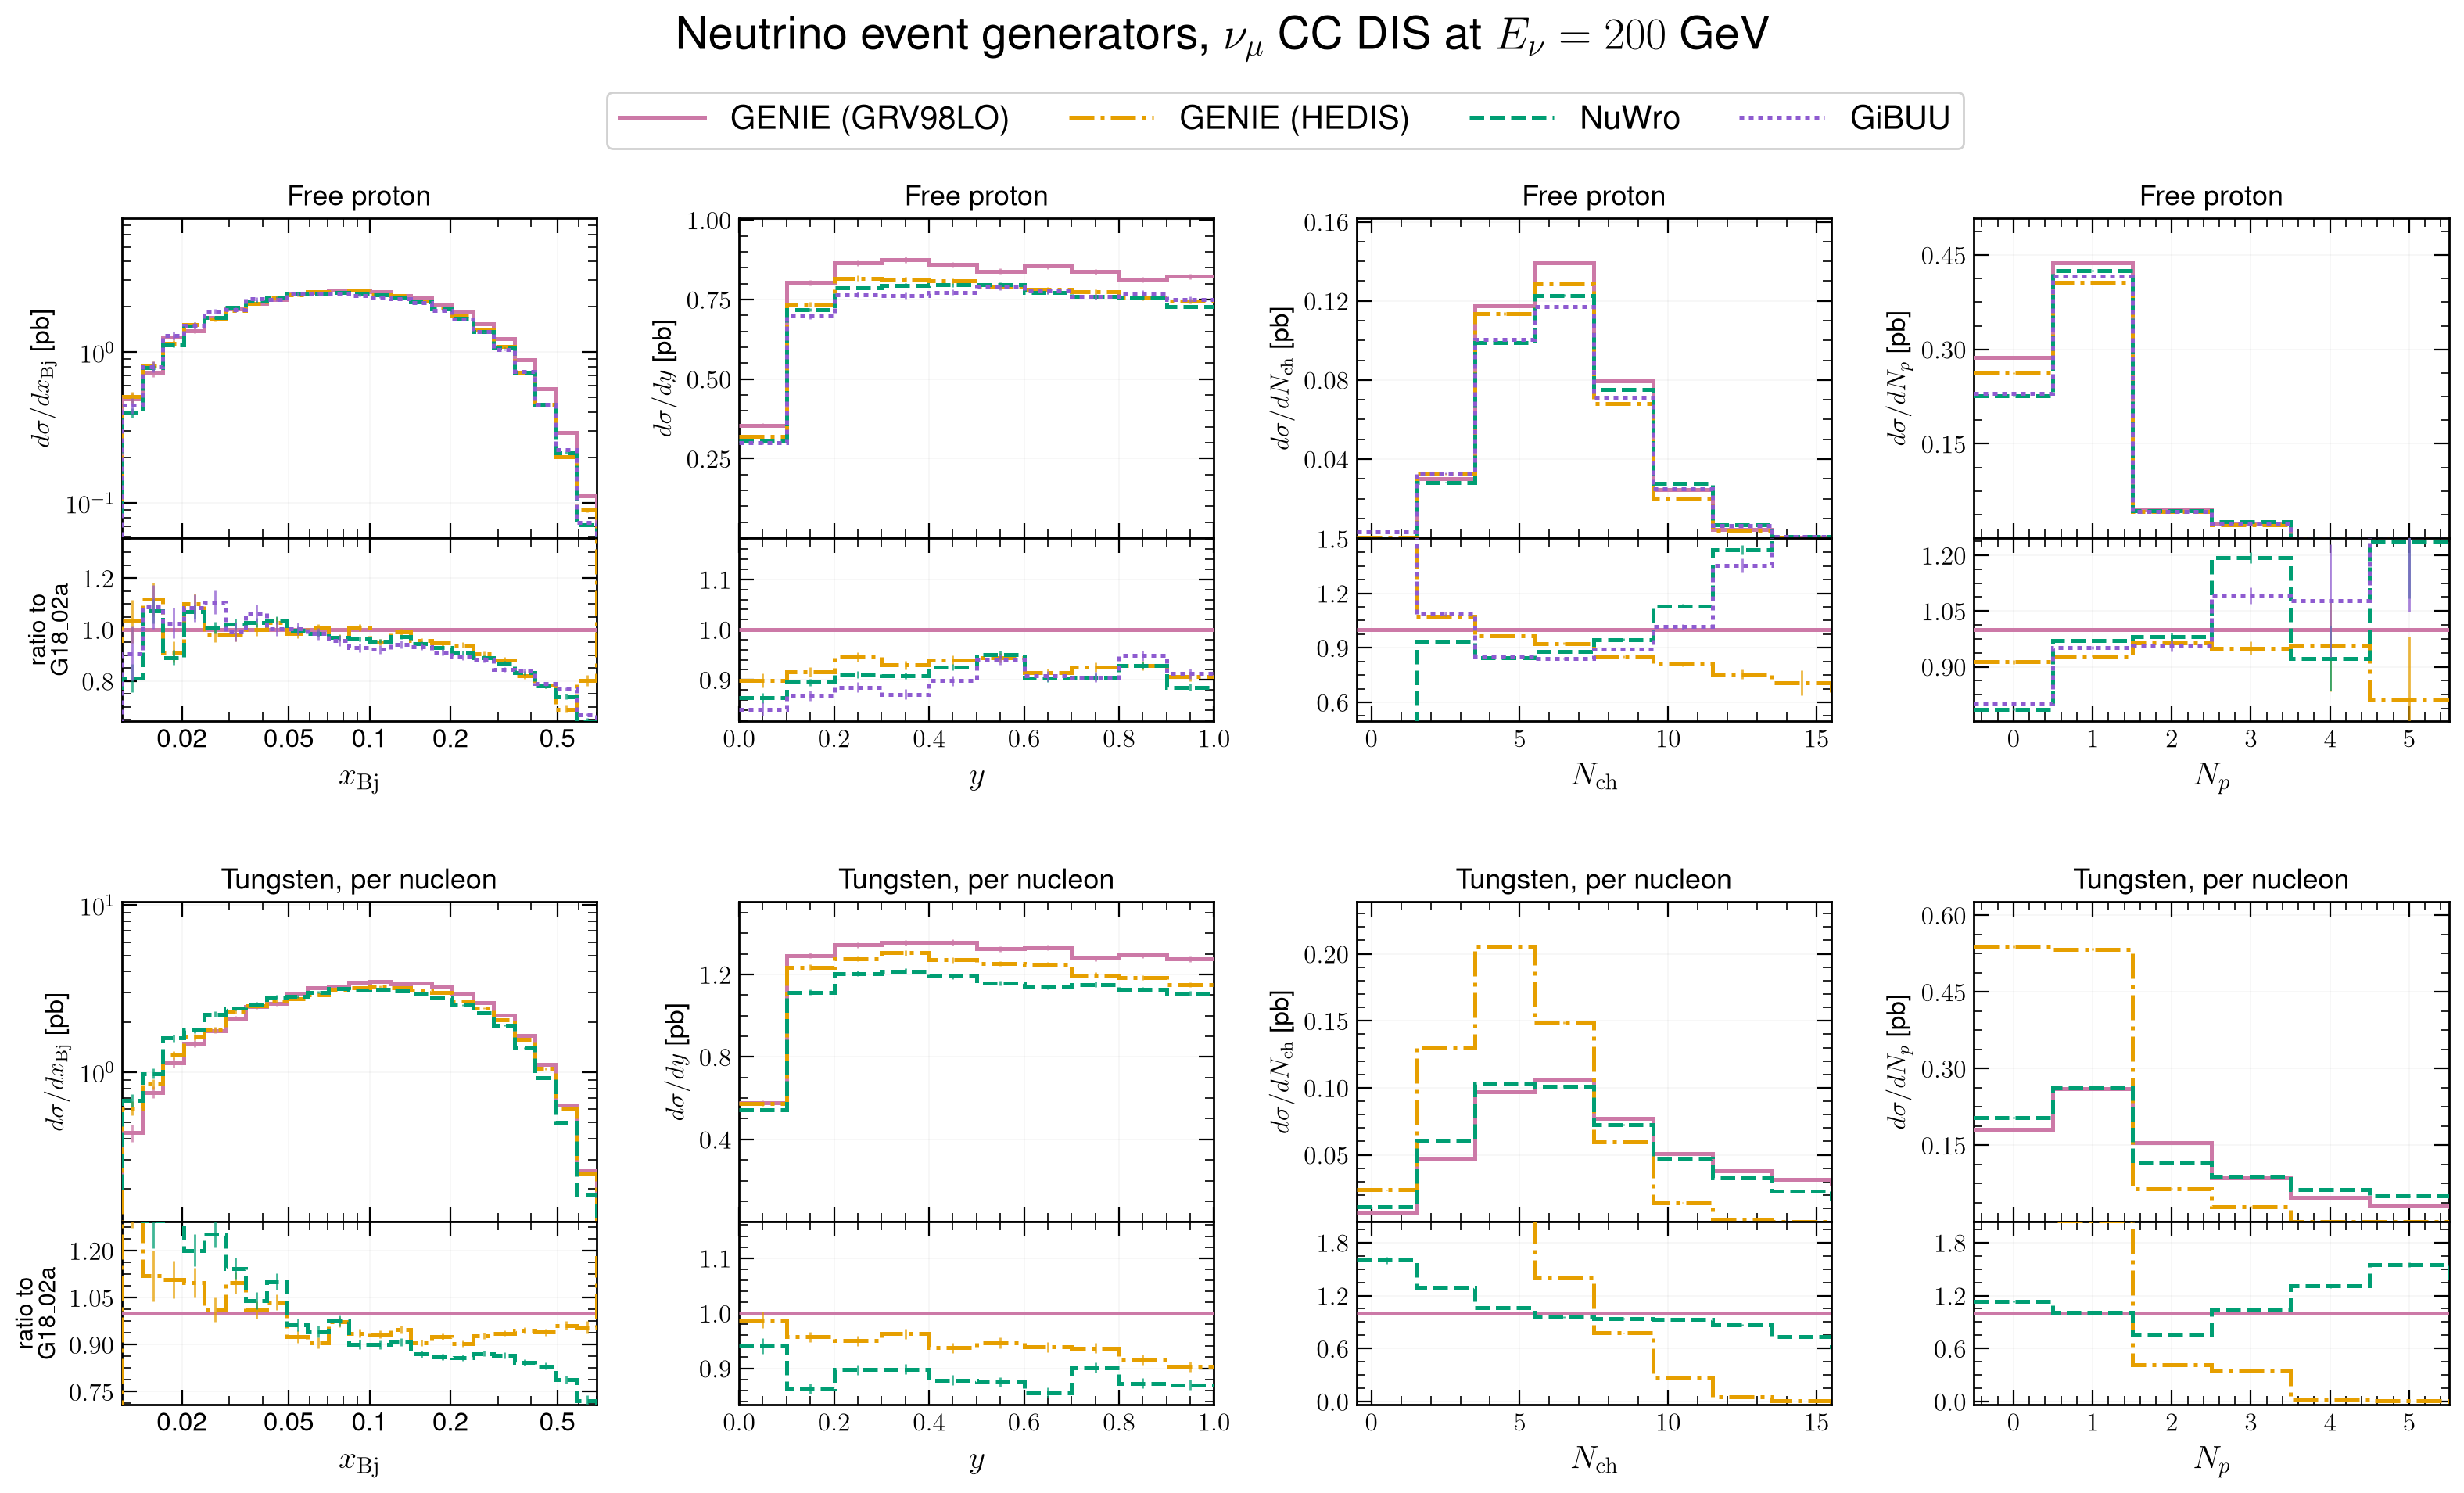
\includegraphics[width=0.99\textwidth]{figures/pp_nu_generators.png}
  \caption{Differential distributions in $x_{\rm Bj}$, $y$, charged-hadron multiplicity $N_{\rm ch}$, and proton multiplicity $N_p$ evaluated in $\nu_\mu$ CC scattering at $E_\nu=200$~GeV in the fiducial region of this benchmark, both on a free proton  target (top) and on a tungsten target (bottom).
  %
  Predictions from three different neutrino MC event generators are compared: \genie (both default {\tt G18\_02a} tune and {\sc\small HEDIS} tune), {\sc\small NuWro} and {\sc\small GiBUU}.
    %
    Note that {\sc\small GiBUU} is shown for the free proton only, since its tungsten transport does not complete at $E_\nu=200$ GeV.
    %
    The bottom panels display the ratio of the various predictions to \genie {\tt G18\_02a}.}
  \label{fig:nugen}
\end{figure}
%%%%%%%%%%%%%%%%%%%%%%%%%%%%%%

On the free proton target, the generators mostly agree on the shapes of the distributions, but one observes large differences in the overall rate: relative to \genie {\tt G18\_02a}, the fiducial cross-section is lower by $9\%$ in {\sc\small NuWro} and $10\%$ in {\sc\small GiBUU}.
%
Larger differences are found on the tungsten target: for example, the intranuclear cascade raises the mean charged multiplicity to $12.5$ in \genie {\tt G18\_02a} and $10.6$ in {\sc\small NuWro}.
%
Note that the {\sc\small HEDIS} tune of \genie  does not simulate final-state interactions, so its hadron multiplicities remain at the free-nucleon level, see also~\cite{Feng:2022inv}.
%
{\sc\small GiBUU} is absent from the tungsten comparison because its hadron transport does not complete at $E_\nu=200$~GeV, and its neutrino module is documented only up to $E_\nu=50$~GeV~\cite{Lalakulich:2012gm}, which limits its applicability to FASER physics.
%
More generally, the nuclear models of the various neutrino generators are tuned to data at much lower energies, and their extrapolation to the TeV energies of FASER neutrinos is in general not expected to work. 